% ==============================================================================
% SECTION 5.4: EMPIRICAL EXERCISE 2: NON-LINEAR DYNAMICS UNDER PERIPHERAL CENTRAL BANK SOLVENCY
% A THRESHOLD VECTOR AUTOREGRESSION APPROACH
% ==============================================================================
% Draft Architecture: First Pass Skeleton and Itemized Contents
% Calibrated to UMass Applied Econometrics & Prose Register Standards

\subsubsection{External Solvency Constraints, Balance-Sheet Dynamics, and Structural Identification}
\label{sec:tvar_specification}

\paragraph{The Solvency Boundary and Macroeconomic Non-Linearity in Dependent Economies.}
The directional precedence tests in Section~\ref{sec:granger_tournament} establish that consumer price inflation exerted persistent predictive feedback on base money expansion, while foreign reserve solvency interacted predictively with base money growth prior to October 1973 (Table~\ref{tab:core_granger_evidence}). Linear vector autoregressions, however, impose time-invariant parameters across fundamentally distinct historical phases. In a financially subordinate open economy lacking international reserve-currency status, convertible foreign exchange reserves ($IR_t$) constitute the ultimate material anchor of domestic policy autonomy. When external reserves are abundant, the monetary authority can buffer domestic employment and intermediate input requirements by absorbing external cost shocks. When foreign exchange reserves are depleted, that insulation mechanism dissolves. 

Under acute foreign exchange scarcity, the transmission of macroeconomic shocks changes discontinuously. Private and state enterprises facing escalating nominal costs for imported spare parts, haul-truck tires, industrial equipment, and basic wage goods could no longer secure foreign letters of credit. To prevent production halts, enterprise illiquidity, and payroll defaults, the Central Bank is compelled into defensive liquidity accommodation. Macroeconomic transmission becomes non-linear: innovations to domestic credit ($g^H_t \to \pi_t$) and nominal price shocks ($\pi_t \to g^H_t$) propagate through distinct structural dynamics depending on whether the monetary authority possesses the hard-currency backing to defend the exchange rate and finance critical imports.

\paragraph{The Solvency Growth Gap: Balance-Sheet Derivation and Economic Interpretation.}
To capture the state of external financial backing, I formalize the Central Bank balance-sheet constraint. Let the Solvency Ratio relative to Central Bank base money liabilities be defined as the dimensionless stock ratio:
\begin{equation}
    S_t \equiv \text{SolvR}^H_t = \frac{F_t}{H_t} = \frac{e_t \cdot IR_t}{H_t \cdot 1000},
    \label{eq:tvar_solv_stock_def}
\end{equation}
where $F_t \equiv e_t \cdot IR_t$ represents the domestic-currency valuation of official international reserves and $H_t$ denotes high-powered reserve money. In discrete time, the stock ratio updates according to the exact multiplicative identity:
\begin{equation}
    S_t = S_{t-1} \exp\left( \frac{g^F_t - g^H_t}{100} \right),
    \label{eq:tvar_stock_flow_update}
\end{equation}
where $g^F_t \equiv \Delta \ln F_t \times 100$ is the monthly growth rate of the domestic-currency reserve stock and $g^H_t \equiv \Delta \ln H_t \times 100$ is the growth rate of high-powered base money. 

Taking natural logarithms and first differences yields the continuous-flow update equation:
\begin{equation}
    \Delta s_t \equiv \Delta \ln S_t \times 100 = g^F_t - g^H_t.
    \label{eq:tvar_solvency_gap_def}
\end{equation}
The variable $\Delta s_t$ defines the \emph{Solvency Growth Gap}. Equation~\eqref{eq:tvar_solvency_gap_def} resolves a major econometric problem. As documented in Section~\ref{sec:tvar_threshold_estimation}, the level stock ratio $S_t$ contains a stochastic trend ($I(1)$), violating the ergodicity requirements of threshold bootstrap inference \citep{Hansen1997,Hansen2000}. By contrast, because $g^F_t$ and $g^H_t$ are stationary percentage changes, their linear combination $\Delta s_t$ is strictly $I(0)$. 

The Solvency Growth Gap also carries clear economic meaning. It tracks the net flow balance between external asset accumulation and domestic liability emission. Because a sovereign monetary authority exercises domestic monopoly over legal tender, central bank insolvency does not describe domestic currency illiquidity; rather, it describes the exhaustion of convertible foreign exchange reserves required to settle balance-of-payments obligations and back domestic high-powered liabilities. When $\Delta s_{t-1} > \gamma$, foreign reserves expand faster than the domestic monetary base, stabilizing the external backing of the currency. When $\Delta s_{t-1} \le \gamma$, domestic credit emission significantly outpaces foreign reserve accumulation. This divergence captures an active entry into conditions of central bank insolvency: the state's capacity to import intermediate goods and food collapses, activating distributive conflict and forcing the monetary authority into defensive accommodation.

\paragraph{The Five-Variable Threshold VAR Specification.}
To model these state-dependent interactions, I specify a five-variable Threshold Vector Autoregression partitioned into a world-money forcing block and a domestic macroeconomic block:
\begin{equation}
    X_t = \begin{bmatrix} g^{gold}_t & \Delta \ln \Theta_t & g^F_t & \pi_{m,t} & g^H_t \end{bmatrix}',
    \label{eq:tvar_variable_vector}
\end{equation}
where $g^{gold}_t$ is the monthly growth rate of the London gold bullion price in US dollars, $\Delta \ln \Theta_t$ is the change in the real structural trade imbalance, $g^F_t$ is the growth rate of domestic-currency international reserves, $\pi_{m,t}$ is monthly consumer price inflation, and $g^H_t$ is Central Bank base money growth. 

The two-regime Threshold VAR with one lag takes the form:
\begin{equation}
    X_t = \mu(s_{t-1}) + A_1(s_{t-1}) X_{t-1} + \varepsilon_t,
    \label{eq:tvar_model_equation}
\end{equation}
where the state indicator $s_{t-1} \in \{0, 1\}$ is governed by the predetermined Solvency Growth Gap relative to the threshold parameter $\gamma$:
\begin{equation}
    s_{t-1} = \begin{cases} 
        1 \quad (\text{Adverse Solvency-Growth State}) & \text{if } \Delta s_{t-1} \le \gamma, \\ 
        0 \quad (\text{Non-Adverse State}) & \text{if } \Delta s_{t-1} > \gamma.
    \end{cases}
    \label{eq:tvar_regime_indicator}
\end{equation}
In Equation~\eqref{eq:tvar_model_equation}, $\mu(s_{t-1})$ is a regime-dependent intercept vector, $A_1(s_{t-1})$ is a $5 \times 5$ regime-dependent coefficient matrix, and $\varepsilon_t$ is a vector of white-noise disturbances with regime-specific covariance matrix $\Sigma(s_{t-1})$.

\paragraph{Structural Identification and International Block Exogeneity.}
Contemporaneous structural identification relies on a Cholesky decomposition of the reduced-form covariance matrix. The recursive ordering aligns with institutional timing and international block exogeneity:
\begin{equation}
    g^{gold}_t \longrightarrow \Delta \ln \Theta_t \longrightarrow g^F_t \longrightarrow \pi_{m,t} \longrightarrow g^H_t.
    \label{eq:tvar_cholesky_order}
\end{equation}
This recursive ordering embeds five institutional timing assumptions:
\begin{enumerate}[leftmargin=*,itemsep=1pt]
    \item Global gold price fluctuations reflect international monetary disruptions, including the breakdown of the Bretton Woods system, and do not respond contemporaneously to Chilean macroeconomic shocks.
    \item The real structural trade imbalance ($\Theta_t$) responds to external terms-of-trade shocks before domestic nominal variables adjust.
    \item The domestic-currency reserve flow ($g^F_t$) adjusts to trade settlements and external credit availability within the month.
    \item Domestic consumer prices ($\pi_{m,t}$) respond within the month to import bottlenecks and foreign exchange shortages, but precede high-powered base money creation.
    \item Central Bank base money emission ($g^H_t$) is ordered last, operating as an endogenous accommodation valve that clears enterprise payments and commercial bank liquidity demands within the month.
\end{enumerate}

To avoid in-sample over-fitting, world gold-price growth is treated as block-exogenous in the recursive ordering. This restriction is supported by the absence of detected domestic feedback in the unrestricted TVAR gold equation ($p > 0.10$, Table~\ref{tab:tvar_estimates}) and by the small-open-economy price-taking assumption. I restrict the lag polynomial of the first equation such that all domestic feedback coefficients equal zero:
\begin{equation}
    \begin{bmatrix} g^{gold}_t \\ X^{dom}_t \end{bmatrix} = \begin{bmatrix} \mu_1(s_{t-1}) \\ \mu_2(s_{t-1}) \end{bmatrix} + \begin{bmatrix} a_{11}(s_{t-1}) & \mathbf{0}_{1 \times 4} \\ A_{21}(s_{t-1}) & A_{22}(s_{t-1}) \end{bmatrix} \begin{bmatrix} g^{gold}_{t-1} \\ X^{dom}_{t-1} \end{bmatrix} + \begin{bmatrix} \varepsilon^{gold}_t \\ \varepsilon^{dom}_t \end{bmatrix},
    \label{eq:tvar_block_exogeneity_matrix}
\end{equation}
where $X^{dom}_t = [\Delta \ln \Theta_t, g^F_t, \pi_{m,t}, g^H_t]'$. 


\subsubsection{Testing for Structural Non-Linearity and Solvency Regime Identification}
\label{sec:tvar_threshold_estimation}

\paragraph{Stationarity of the Solvency Flow Gap versus Wandering Reserve Stocks.}
Standard threshold autoregressive models require the transition variable to follow a strictly stationary ergodic process \citep{Hansen1997,Hansen2000}. If a threshold variable contains a stochastic trend ($I(1)$), its empirical density does not cross the boundary with stationary frequency. The series instead wanders away from the threshold for extended historical intervals. Under non-stationarity, standard asymptotic inference collapses, and the threshold search risks identifying spurious chronological breaks rather than recurrent economic states.

Table~\ref{tab:solvency_unit_root} reports the complete stationarity diagnostic battery for both the level stock ratio ($S_t$) and the dynamic flow gap ($\Delta s_t$). For the level solvency ratio, the Augmented Dickey--Fuller test statistic is $-0.564$ ($p = 0.978$), and the Phillips--Perron test statistic is $-1.291$ ($p = 0.983$). Both tests fail to reject the unit-root null hypothesis. The KPSS test likewise rejects the null of level stationarity ($1.726$, $p < 0.01$) and trend stationarity ($0.494$, $p < 0.01$). The level stock $S_t$ is unambiguously an $I(1)$ process.

\begin{table}[htbp]
\centering
\small
\renewcommand{\arraystretch}{0.92}
\caption{Integration Order Diagnostics for Central Bank Solvency Variables (1960:01--1980:12)}
\label{tab:solvency_unit_root}
\label{tab:tab03_solvency_unit_root}
\resizebox{\textwidth}{!}{%
\begin{tabular}{lccccccr}
\toprule
\textbf{Variable / Series} & \multicolumn{2}{c}{\textbf{ADF Test}} & \multicolumn{2}{c}{\textbf{Phillips--Perron}} & \multicolumn{2}{c}{\textbf{KPSS Test}} & \textbf{Order / Classification} \\
\cmidrule(lr){2-3} \cmidrule(lr){4-5} \cmidrule(lr){6-7}
 & \textbf{Stat.} & \textbf{$p$-val} & \textbf{Stat.} & \textbf{$p$-val} & \textbf{Level} & \textbf{Trend} & \\
\midrule
Solvency Ratio ($S_t$, levels) & -0.564 & 0.978 & -1.291 & 0.983 & 1.726$^{***}$ & 0.494$^{***}$ & $I(1)$ (Non-stationary) \\
Solvency Growth Gap ($\Delta s_t$, diff.) & -4.941$^{***}$ & $<0.01$ & -14.011$^{***}$ & $<0.01$ & 0.570$^{*}$ & 0.082 & $I(0)$ (Stationary) \\
\bottomrule
\end{tabular}%
}
\begin{minipage}{\textwidth}
\vspace{0.4em}
\footnotesize \textit{Notes:} Monthly series spanning 1960:01--1980:12 ($N=250$). The level solvency ratio is defined as $S_t \equiv (e_t \cdot IR_t) / (H_t \cdot 1000)$. The Solvency Growth Gap is defined as the exact log difference $\Delta s_t \equiv g^F_t - g^H_t = \Delta \ln S_t \times 100$. Augmented Dickey--Fuller (ADF) tests estimated with constant drift; lag orders selected via Schwarz Bayesian Information Criterion (SBIC). Phillips--Perron (PP) tests employ Newey--West Bartlett kernel bandwidth. For ADF and PP, the null hypothesis is a unit root ($I(1)$); for KPSS, the null hypothesis is stationarity ($I(0)$). Significance: $^{***} p < 0.01$, $^{**} p < 0.05$, $^{*} p < 0.10$. The test battery indicates that the level stock $S_t$ contains a stochastic trend (failing to reject the unit-root null and rejecting KPSS stationarity), whereas the flow growth gap $\Delta s_t$ rejects the unit root and fails to reject trend stationarity, providing evidence consistent with covariance stationarity ($I(0)$) and satisfying the ergodicity preconditions for \citet{Hansen1997,Hansen2000} threshold estimation.
\end{minipage}
\end{table}


By contrast, evaluating the first-differenced Solvency Growth Gap ($\Delta s_t \equiv g^F_t - g^H_t$) yields an Augmented Dickey--Fuller statistic of $-4.941$ ($p < 0.01$) and a Phillips--Perron statistic of $-14.011$ ($p < 0.01$). Both reject the unit-root null hypothesis at the 1\% level. The KPSS test statistic is $0.570$, failing to reject the stationarity null at the 1\% level. The Solvency Growth Gap is stationary ($I(0)$). Specifying $\Delta s_{t-1}$ as the predetermined threshold variable satisfies the relevant integration-order requirement for Hansen threshold estimation.

\paragraph{Concentrated Least Squares Estimation and Rejection of Linearity.}
Having established the stationarity of the transition variable, I estimate the unknown threshold parameter $\gamma$ using concentrated least squares. The estimation algorithm minimizes the determinant of the residual covariance matrix, $\det(\hat{\Sigma}(\gamma))$, across the trimmed empirical support of $\Delta s_{t-1}$. Following \citet{Hansen1999}, I apply a trimming parameter of $\tau = 0.15$, ensuring that every identified regime contains a minimum of 37 monthly observations from the full sample of $N=250$.

Because the threshold parameter $\gamma$ is unidentified under the linear null hypothesis ($H_0: A_1(0) = A_1(1)$), standard likelihood ratio tests follow non-standard asymptotic distributions. To obtain valid inference, I follow \citet{Hansen1999} and implement the Supremum Likelihood Ratio (Sup-LR) test using a residual bootstrap with $B = 1{,}000$ replications. The bootstrap resampling procedure preserves cross-equation contemporaneous error correlation while imposing the linear null restriction.

The resulting test statistic is $\text{Sup-LR} = 112.10$, corresponding to a bootstrap $p$-value of $p = 0.0010$. The bootstrap threshold test rejects the constant-parameter linear specification in favor of the estimated threshold alternative, providing evidence against parameter constancy across the solvency growth gap dimension. The rate at which the monetary authority accumulates foreign reserves relative to domestic liabilities alters the macroeconomic propagation mechanism.

\paragraph{Regime Partition Discipline: Isolating Conditions of Central Bank Insolvency.}
To identify the number of operative regimes, I conduct an unrestricted two-dimensional grid search across candidate thresholds $(\gamma_1, \gamma_2)$. The algorithm isolates two global structural breaks at $\hat{\gamma}_1 = -4.61\%$ and $\hat{\gamma}_2 = +20.87\%$. This partition divides the 250 monthly observations into three distinct economic states:
\begin{enumerate}[leftmargin=*,itemsep=1pt]
    \item \emph{Adverse Solvency-Growth State} ($\Delta s_{t-1} \le -4.61\%$, $N_1 = 100$ months, $40.0\%$ of the sample, reflecting conditions of central-bank insolvency): Base money expansion systematically outpaces foreign reserve accumulation by more than 4.6 percentage points per month.
    \item \emph{Intermediate State} ($-4.61\% < \Delta s_{t-1} \le +20.87\%$, $N_2 = 111$ months, $44.4\%$ of the sample): External reserve growth and domestic credit creation remain within bounded historical corridors.
    \item \emph{High Reserve Accumulation State} ($\Delta s_{t-1} > +20.87\%$, $N_3 = 38$ months, $15.2\%$ of the sample): Rapid foreign exchange accumulation driven by world commodity windfalls.
\end{enumerate}

Although the three-state model captures the upper tail of commodity windfalls, finite-sample constraints dictate careful specification discipline \citep{Hansen1999,Afonso2018}. In a five-variable vector autoregression, each equation requires estimating 7 parameters at $p=1$ and 12 parameters at $p=2$. With only $N_3 = 38$ observations in the high-accumulation regime, degrees of freedom contract to 31 (at $p=1$) and 26 (at $p=2$). Estimating dynamic Generalized Impulse Response Functions on such a small partition induces parameter instability and inflated bootstrap variance.

Because the central objective of this chapter is to examine macroeconomic adjustment under acute foreign exchange depletion rather than commodity windfalls, I adopt a two-regime baseline specification. The model isolates the adverse solvency-growth state ($\Delta s_{t-1} \le -4.615\%$, $N = 100$, degrees of freedom $df = 93$) and pools the remaining observations into a unified non-adverse solvency-growth state ($\Delta s_{t-1} > -4.615\%$, $N = 145$, degrees of freedom $df = 138$). This baseline balances degrees-of-freedom discipline with structural precision, providing a robust empirical foundation for dynamic simulation.

Figure~\ref{fig:regime_timeline} plots the resulting endogenous regime classification across the 1960--1980 timeline, contrasting the persistent level solvency stock ($S_t$) with the stationary flow gap ($\Delta s_t$) and the estimated structural threshold ($\hat{\gamma}_1 = -4.615\%$).

\begin{figure}[htbp]
\centering
\begin{subfigure}[b]{0.49\textwidth}
    \centering
    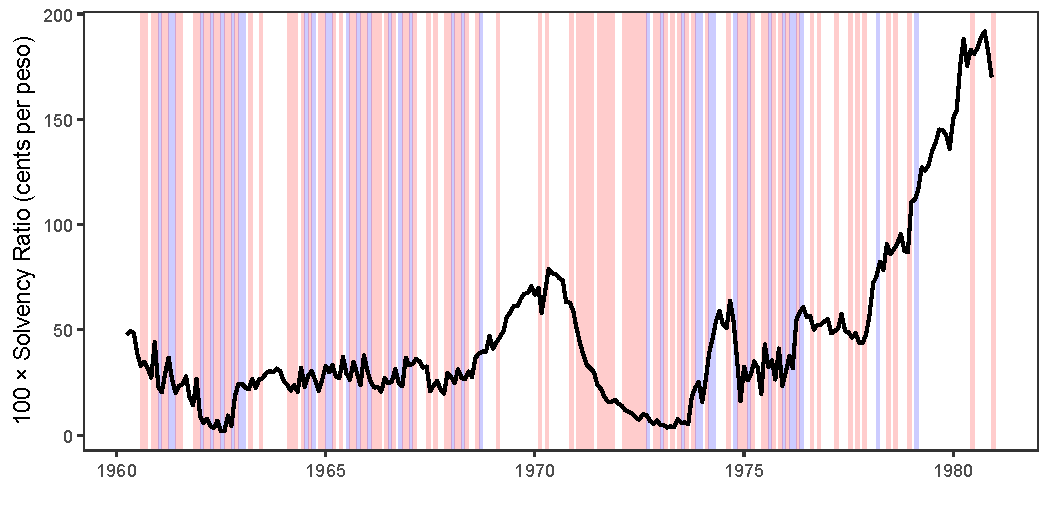
\includegraphics[width=\textwidth]{figures/regime_timeline_level.pdf}
    \caption{Solvency Ratio Stock ($100 \times S_t$)}
    \label{fig:regime_timeline_stock}
\end{subfigure}
\hfill
\begin{subfigure}[b]{0.49\textwidth}
    \centering
    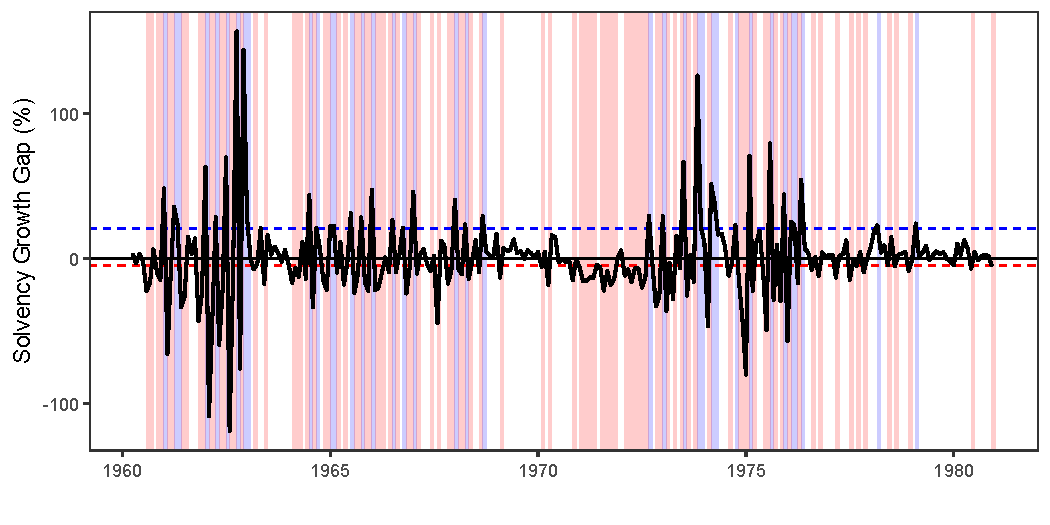
\includegraphics[width=\textwidth]{figures/regime_timeline_gap.pdf}
    \caption{Solvency Growth Gap Flow ($\Delta s_t$)}
    \label{fig:regime_timeline_gap}
\end{subfigure}
\caption{Central Bank Solvency Ratio and Solvency Growth Gap, 1960--1980}
\label{fig:regime_timeline}
\begin{minipage}{\textwidth}
    \vspace{0.3em}
    \footnotesize \textbf{Notes:} \textbf{Panel (A)} displays the monthly Central Bank Solvency Ratio stock ($100 \times S_t \equiv 100 \times [e_t IR_t / (H_t \cdot 1000)]$, expressed as cents per peso). \textbf{Panel (B)} displays the predetermined threshold variable, the Solvency Growth Gap ($\Delta s_t \equiv g^F_t - g^H_t = \Delta \ln S_t \times 100$). Shaded areas distinguish the exploratory three-state diagnostic partition identified by the Concentrated Least Squares grid search: red shading marks the adverse solvency-growth state ($\Delta s_{t-1} \le -4.615\%$, $N=100$), blue shading marks the exploratory upper-tail reserve-accumulation state ($\Delta s_{t-1} > +20.878\%$, $N=38$), and unshaded areas denote the intermediate partition ($N=111$). For econometric estimation and dynamic GIRF simulations, the baseline TVAR pools the two non-adverse partitions into a single unified non-adverse state ($\Delta s_{t-1} > -4.615\%$, $N=145$). The dashed horizontal line in Panel (B) marks the estimated structural threshold ($\hat{\gamma} = -4.615\%$). Data sources: Central Bank of Chile (BCCh) monthly balance sheets (1960:01--1980:12, $N=250$).
\end{minipage}
\end{figure}


\subsubsection{Historical Regime Chronology and the Unidad Popular Trajectory}
\label{sec:tvar_regime_chronology}

\paragraph{Stock-Flow Dynamics: Reserve Exhaustion versus Flow Stabilization.}
The dual-panel trajectory in Figure~\ref{fig:regime_timeline} clarifies the analytical distinction between the level stock of international solvency ($S_t$) and its dynamic flow gap ($\Delta s_t$). Panel~(A) shows that the ratio of official international reserves to Central Bank base money liabilities dropped precipitously in late 1970 and remained near zero throughout 1971--1978. A static stock threshold would classify this entire eight-year window as a single continuous insolvency regime. Such a classification fails to distinguish between active balance-of-payments insolvency and the post-1974 orthodox stabilization under low foreign exchange reserves. Under the military dictatorship, drastic fiscal retrenchment and the contraction of real wages stabilized the flow gap ($\Delta s_t > 0$), despite the depleted stock of reserves.

Panel~(B) demonstrates why the Solvency Growth Gap operates as the true transition trigger. The structural break occurs not when reserve stocks are low in absolute terms, but when base money creation persistently outpaces foreign reserve accumulation. By taking the logarithmic first difference ($\Delta s_t \equiv g^F_t - g^H_t$), the threshold condition $\Delta s_{t-1} \le -4.615\%$ isolates the rate of net reserve depletion. When this gap turns sharply negative, domestic liquidity creation dilutes external reserve backing. The state loses the foreign exchange required to maintain import parities, unanchoring domestic price stability.

\paragraph{Endogenous Dating of the Unidad Popular Macroeconomic Trajectory.}
Without imposing calendar dummies or political intervention dates, the threshold condition $\Delta s_{t-1} \le -4.615\%$ autonomously classifies the critical junctures of the Unidad Popular administration (1970--1973) into the adverse solvency-growth state (reflecting conditions of central-bank insolvency). The mathematical threshold search identifies five distinct historical episodes:
\begin{enumerate}[leftmargin=*,itemsep=1pt]
    \item \emph{November 1970:} Immediate post-electoral capital flight following Salvador Allende's victory triggers an initial gap of $\Delta s_t = -15.18\%$, reflecting commercial bank deposit withdrawals and private asset flight abroad.
    \item \emph{January--May 1971:} The initial redistributive expansion under the Vuskovi\'c Plan drives the growth gap to between $-13\%$ and $-15\%$. High-powered money emission financed public enterprise wage increases while foreign reserves remained stable, initiating the dilution of reserve coverage.
    \item \emph{July--November 1971:} International commercial banks suspended short-term trade credit lines, and US export credit dried up \citep{Stallings1978,DeVylder1976}. The growth gap plunged between $-6\%$ and $-22\%$, reflecting the exhaustion of foreign exchange buffers.
    \item \emph{November--December 1972:} In the aftermath of the October 1972 employer lockout and transport strike \citep[see][]{Casals2021}, the Central Bank extended emergency credit to keep nationalized enterprises operating. The flow gap collapsed to $-26.4\%$ in November and $-33.1\%$ in December.
    \item \emph{February, April, and August 1973:} The final phase of the administration witnessed acute supply bottlenecks for imported spare parts, haul-truck tires, and wheat. With reserves exhausted, the gap reached $-25\%$ to $-36\%$, locking the economy into an accelerating inflation regime.
\end{enumerate}

\paragraph{Endogenous Accommodation versus the Orthodox Narrative of Policy Pathology.}
These empirical findings challenge orthodox accounts of the Chilean transition \citep{DornbuschEdwards1990,Edwards2024}. Mainstream interpretations treat the Unidad Popular inflation as an unforced episode of macroeconomic populism driven by autonomous deficit monetization. In that narrative, monetary policy operates as an independent prime mover unconstrained by external balances. 

The threshold model reveals an alternate institutional mechanism. Monetary emission accelerated defensively to finance enterprise payrolls and purchase essential inputs under strict foreign credit constraints. When foreign commercial banks cut off short-term letters of credit, the state could no longer import intermediate capital goods or food to stabilize domestic markets. Distributive conflict over real income could no longer be pacified through external supply. Under acute reserve depletion, the Central Bank entered an endogenous liquidity accommodation dynamic: price increases required nominal credit expansion to avert enterprise liquidation, which eroded external solvency and amplified inflationary expectations.


\subsubsection{Regime-Dependent Parameter Estimates and Accommodation Dynamics}
\label{sec:tvar_parameter_estimates}

\begin{table}[htbp]
\centering
\small
\renewcommand{\arraystretch}{0.90}
\caption{Regime-Dependent TVAR Parameter Estimates across Solvency Regimes (1960--1980)}
\label{tab:tvar_estimates}
\label{tab:tab04_tvar_estimates}
\resizebox{\textwidth}{!}{%
\begin{tabular}{lccccc}
\toprule
\textbf{Lagged Regressor} & \multicolumn{5}{c}{\textbf{Dependent System Variables ($X_t$)}} \\
\cmidrule(lr){2-6}
 & \textbf{Gold ($g^{gold}_t$)} & \textbf{Imbalance ($\Delta \ln \Theta_t$)} & \textbf{Reserves ($g^F_t$)} & \textbf{Inflation ($\pi_{m,t}$)} & \textbf{Money ($g^H_t$)} \\
\midrule
\multicolumn{6}{l}{\textbf{Panel A: Adverse Solvency-Growth State} ($\Delta s_{t-1} \le -4.615\%$, $N_1 = 100$ months)} \\
\midrule
Constant & 0.636 & -3.720 & 3.388 & -0.300 & 1.893$^{*}$ \\
World Gold Price ($g^{gold}_{t-1}$) & 0.625$^{***}$ & 0.378 & -0.494 & 0.197$^{**}$ & 0.151 \\
Structural Imbalance ($\Delta \ln \Theta_{t-1}$) & --- & -0.188$^{*}$ & --- & 0.010 & --- \\
Reserve Growth ($g^F_{t-1}$) & --- & --- & -0.181 & -0.016 & -0.042 \\
CPI Inflation ($\pi_{m,t-1}$) & --- & --- & 0.512 & 0.684$^{***}$ & 0.581$^{***}$ \\
Base Money Growth ($g^H_{t-1}$) & --- & --- & 0.938 & 0.166$^{***}$ & 0.058 \\
Price Decontrol Dummy ($D_{oct73}$) & -1.225 & 62.520 & 111.026$^{***}$ & 76.213$^{***}$ & -2.775 \\
\midrule
\multicolumn{6}{l}{\textbf{Panel B: Non-Adverse Solvency-Growth State} ($\Delta s_{t-1} > -4.615\%$, $N_2 = 145$ months)} \\
\midrule
Constant & 0.579 & 1.836 & 1.848 & 2.218$^{***}$ & 3.300$^{***}$ \\
World Gold Price ($g^{gold}_{t-1}$) & 0.339$^{***}$ & -1.128$^{**}$ & 0.312 & -0.013 & -0.034 \\
Structural Imbalance ($\Delta \ln \Theta_{t-1}$) & --- & -0.629$^{***}$ & --- & -0.009 & --- \\
Reserve Growth ($g^F_{t-1}$) & --- & --- & -0.355$^{***}$ & -0.014 & 0.006 \\
CPI Inflation ($\pi_{m,t-1}$) & --- & --- & 1.114$^{***}$ & 0.275$^{***}$ & 0.236$^{***}$ \\
Base Money Growth ($g^H_{t-1}$) & --- & --- & -0.173 & 0.240$^{***}$ & 0.115 \\
\bottomrule
\end{tabular}%
}
\begin{minipage}{\textwidth}
\vspace{0.4em}
\footnotesize \textit{Notes:} Monthly series spanning 1960:01--1980:12 ($N=250$, effective sample $T=245$). Conditional Least Squares (CLS) estimates of the five-variable TVAR(1) conditioned on the predetermined Solvency Growth Gap $\Delta s_{t-1} \equiv g^F_{t-1} - g^H_{t-1}$ at the structural threshold $\hat{\gamma} = -4.615\%$. Significance: $^{***} p < 0.01$, $^{**} p < 0.05$, $^{*} p < 0.10$. Dashes (---) denote structural exclusion restrictions: (i) world gold is block exogenous to domestic Chilean variables ($a_{12} = a_{13} = a_{14} = a_{15} = 0$); (ii) real structural imbalance ($\Delta \ln \Theta_t$) is exogenous to domestic feedback ($a_{23} = a_{24} = a_{25} = 0$); and (iii) lagged structural imbalance ($\Delta \ln \Theta_{t-1}$) is excluded from central bank solvency equations ($g^F_t$ and $g^H_t$, $a_{32} = a_{52} = 0$), in accordance with the institutional transmission structure and Latin American structuralist theory. The one-off price decontrol dummy $D_{oct73}$ (Decree Law 522) in Panel A controls for the October 1973 administrative price decontrol and foreign exchange revaluation shock.
\end{minipage}
\end{table}


\paragraph{Equation Estimates and Small-Economy Structural Restrictions.}
Table~\ref{tab:tvar_estimates} reports the conditional least squares parameter estimates for the five-variable Threshold VAR across the adverse solvency-growth state (reflecting conditions of central-bank insolvency) and the non-adverse state. Equation-by-equation estimation isolates the dynamic interactions among world gold prices, the structural import imbalance, international reserves, consumer price inflation, and base money. Following the identification strategy in Section~\ref{sec:tvar_specification}, I impose three structural exclusion restrictions. First, block exogeneity is imposed on the world gold price equation by setting domestic feedback coefficients to zero ($a_{12} = a_{13} = a_{14} = a_{15} = 0$), reflecting Chile's status as a small open economy and price taker in international gold and credit markets; in unrestricted estimations, lagged domestic variables ($\pi_{m,t-1}, g^H_{t-1}, g^F_{t-1}, \Delta \ln \Theta_{t-1}$) are individually and jointly insignificant in the gold equation ($p > 0.10$). Second, domestic feedbacks are excluded from the real structural imbalance equation ($\Delta \ln \Theta_t$), capturing import purchasing capacity constraints as driven by terms of trade and historical import dependence. Third, lagged structural imbalance ($\Delta \ln \Theta_{t-1}$) is excluded from the foreign reserve flow ($g^F_t$) and base money creation ($g^H_t$) equations based on the institutional structure of transmission: structural trade bottlenecks do not mechanically alter reserve flows or print money directly, but operate sequentially through domestic price formation ($\Delta \ln \Theta \to \pi_m$), which the monetary authority accommodates ($\pi_m \to g^H$). Supplementary linear exploratory estimations in Appendix~\ref{app:linear_var_diagnostics} do not provide evidence against this exclusion. In Panel~A, the one-off dummy $D_{oct73}$ controls for the October 1973 administrative price decontrol and foreign exchange revaluation shock under Decree Law 522.

\paragraph{Three Structural Transmission Shifts across Solvency Regimes.}
Comparing parameter estimates across regimes reveals three fundamental structural shifts in the inflation and monetary transmission mechanisms. First, monetary accommodation surges when foreign solvency collapses. In the base money equation ($g^H_t$), the coefficient on lagged inflation ($\pi_{m,t-1}$) rises from $0.236$ ($t = 3.63, p < 0.01$) in the non-adverse state to $0.581$ ($t = 3.90, p < 0.01$) under the adverse solvency-growth state. The accommodation response more than doubles. In the non-adverse state, a 10 percentage point increase in monthly inflation induced only a modest 2.4 percentage point adjustment in base money growth. In the adverse state, that same inflation pulse generated a 5.8 percentage point expansion in base money. When foreign commercial banks canceled short-term credit lines and letters of credit, enterprises could not import replacement machinery or raw materials on deferred payment terms. The Central Bank expanded base money defensively to cover soaring payrolls and working-capital requirements, preventing enterprise illiquidity and factory closures.

Second, price persistence escalates sharply under conditions of central bank insolvency. In the inflation equation ($\pi_{m,t}$), the autoregressive coefficient on lagged inflation rises from $\hat{\beta} = 0.275$ ($t = 6.37, p < 0.01$) in the non-adverse state to $\hat{\beta} = 0.684$ ($t = 8.68, p < 0.01$) in the adverse solvency-growth state. The non-adverse state displays rapid mean reversion. In contrast, the adverse solvency-growth state exhibits near-unit-root inflation inertia. With external reserves depleted, the state could no longer import food or wage goods to stabilize retail prices. Domestic firms engaged in defensive markup revisions, anticipating future currency depreciations and shortages of imported haul-truck tires and spare parts. Speculative hoarding and retail shortages dismantled official price ceilings, cementing self-fulfilling inflation dynamics.

Third, international price pass-through unshields domestic markets during solvency distress. The transmission coefficient from world gold price growth to domestic inflation ($g^{gold}_{t-1} \to \pi_{m,t}$) is economically small and statistically indistinguishable from zero in the non-adverse state ($\hat{\beta} = -0.013, t = -0.23, p = 0.818$). In the adverse solvency-growth state, this pass-through jumps to $\hat{\beta} = +0.197$ ($t = 2.33, p < 0.05$). When foreign exchange reserves are adequate, the Central Bank absorbs external nominal volatility through its reserve buffer and managed import quotas. In the adverse state, this external buffer disintegrates. International monetary instability and US dollar devaluations pass directly into domestic consumer prices through escalating import costs for copper mining equipment and industrial fuels.

\paragraph{Parameter Stability across Threshold Specifications.}
The identified structural shifts remain invariant to the exact placement of the insolvency threshold. The notes to Table~\ref{tab:tvar_estimates} compare the baseline estimates ($\hat{\gamma} = -4.615\%, N_1 = 100$) against the negative-constrained grid search optimum ($\hat{\gamma} = -3.58\%, N_1 = 104$). Across both sample partitions, the key behavioral parameters remain stable. The defensive accommodation coefficient ($\pi_{m,t-1} \to g^H_t$) changes only from $0.581$ to $0.584$ (both $p < 0.01$). Autoregressive inflation persistence shifts from $0.684$ to $0.689$ (both $p < 0.01$). World gold pass-through remains positive and significant ($0.197$ at $p < 0.05$ versus $0.167$ at $p < 0.10$). This parameter stability indicates that the estimated threshold behavior and qualitative regime differences are preserved across alternative threshold locations rather than being driven by local sample sensitivity.



\subsubsection{Dynamic Multipliers and Regime-Dependent Shock Propagation}
\label{sec:tvar_girf_multipliers}

\paragraph{Dynamic Shock Propagation under Endogenous State Transitions.}
To trace how structural shocks propagate dynamically across regimes, the linear impulse response framework must be generalized. In linear vector autoregressions, orthogonalized impulse response functions derived from a Cholesky decomposition assume invariant transmission parameters and history independence. In a Threshold VAR, dynamic propagation depends on the initial state of Central Bank solvency ($\Delta s_{t-1}$), the sign and magnitude of structural innovations to credit or import costs, and the endogenous probability of transitioning across regimes over the forecast horizon.

Following \citet{KoopPesaranPotter1996}, I define the Generalized Impulse Response Function (GIRF) as the expectation of the system's trajectory conditional on a specific structural shock $\nu_t$ and historical information set $\Omega_{t-1}$, relative to an unshocked baseline trajectory:
\begin{equation}
    \text{GIRF}_X(h, \nu_t, \Omega_{t-1}) = \mathbb{E}\left[ X_{t+h} \mid \nu_t, \Omega_{t-1} \right] - \mathbb{E}\left[ X_{t+h} \mid \Omega_{t-1} \right],
    \label{eq:tvar_girf_def}
\end{equation}
where $h = 0, 1, \dots, H$ denotes the forecast horizon. The conditional expectations in Equation~\eqref{eq:tvar_girf_def} are evaluated by Monte Carlo integration. For each regime, I sample $S = 250$ historical starting vectors $\Omega_{t-1}$ belonging to that regime. From each history, the system is simulated forward over $H = 12$ months by drawing $R = 500$ sequences of bootstrap residuals with replacement, preserving empirical non-Gaussianity and contemporaneous residual cross-correlations. In each simulation step, base money growth ($g^H_{t+j}$) and reserve growth ($g^F_{t+j}$) update the endogenous Solvency Growth Gap ($\Delta s_{t+j} \equiv g^F_{t+j} - g^H_{t+j}$), allowing the system to transition endogenously between the adverse solvency-growth state (reflecting conditions of central-bank insolvency) and the non-adverse state.

\paragraph{Evaluating Asymmetric Multipliers across Solvency States.}
To evaluate whether transmission asymmetries between solvency regimes are statistically significant, I formulate a point-wise dynamic multiplier difference test across forecast horizons:
\begin{equation}
    H_0: \Delta_{i,j}(h) \equiv \text{GIRF}_{i,j}^{\text{Insolv}}(h) - \text{GIRF}_{i,j}^{\text{Normal}}(h) = 0,
    \label{eq:tvar_multiplier_diff_test}
\end{equation}
where $\Delta_{i,j}(h)$ measures the difference in the dynamic response of variable $i$ to a structural shock in variable $j$ between the adverse solvency-growth state (reflecting conditions of central-bank insolvency) and the non-adverse state at horizon $h$. Confidence intervals (90\% and 95\%) for the multiplier differences are computed via the percentile bootstrap across the resampled histories. The complete set of 16 empirical impulse response pathways, dynamic multiplier difference tests across all 25 shock-response pairs, and endogenous regime-switching probability matrices are documented in Appendix~\ref{app:tvar_girf_atlas}.

\paragraph{Forward Transmission versus Reverse Accommodation: Dynamic Multiplier Analysis.}
Contrasting the speed, scale, and persistence of forward versus reverse transmission directly evaluates the central theoretical dispute of this chapter. Orthodox accounts \citep{DornbuschEdwards1990,Edwards2024} argue that discretionary high-powered money creation functioned as the primary autonomous driver of the Chilean inflation. The dynamic Generalized Impulse Response trajectories in Figure~\ref{fig:tvar_girf_tournament} are difficult to reconcile with that premise. 

Forward monetary transmission ($g^H \to \pi_m$, Panel~A) operates with modest magnitude and gradual momentum. In the adverse solvency-growth state (reflecting conditions of central-bank insolvency), a one-standard-deviation innovation to base money growth increases monthly consumer price inflation by a peak of $0.966$ percentage points at month 1 ($h=1$). Statistical significance persists across nine consecutive months ($h=1$ to $9$), generating a cumulative price acceleration of $3.550$ percentage points over the year. In the non-adverse solvency-growth state, the response peaks at $1.256$ percentage points at month 1 and remains significant for six months ($h=1$ to $6$), with a cumulative expansion of $2.215$ percentage points. The dynamic multiplier difference ($\Delta_{g^H \to \pi_m}(h)$) is statistically significant across months 4 through 8, peaking at $+0.313$ percentage points at month 3. Forward transmission operates with measurable persistence, but its response profile is constrained. High-powered money emission does not induce an instantaneous hyperinflationary explosion.

\begin{figure}[htbp]
\centering
\begin{subfigure}[b]{0.49\textwidth}
    \centering
    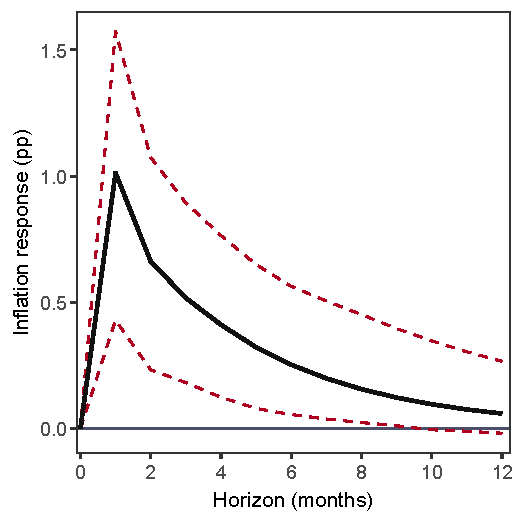
\includegraphics[width=\textwidth]{figures/tvar_girf_forward_money.pdf}
    \caption{Forward Monetary Transmission ($g^H \to \pi_m$)}
    \label{fig:tvar_girf_forward_money}
\end{subfigure}
\hfill
\begin{subfigure}[b]{0.49\textwidth}
    \centering
    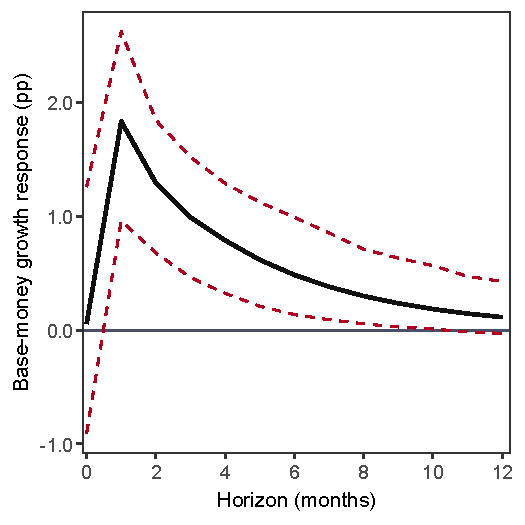
\includegraphics[width=\textwidth]{figures/tvar_girf_reverse_accom.pdf}
    \caption{Reverse Accommodation ($\pi_m \to g^H$)}
    \label{fig:tvar_girf_reverse_accom}
\end{subfigure}
\caption{Dynamic Multipliers under Adverse Solvency-Growth Conditions: Forward Transmission versus Reverse Accommodation}
\label{fig:tvar_girf_tournament}
\begin{minipage}{\textwidth}
    \vspace{0.3em}
    \footnotesize \textbf{Notes:} Generalized Impulse Response Functions (GIRFs) over a 12-month horizon in the adverse solvency-growth state ($\Delta s_{t-1} \le -4.615\%$, reflecting conditions of central-bank insolvency). Solid black lines trace median bootstrap responses to a one-standard-deviation structural innovation; dashed crimson lines represent 90\% empirical bootstrap confidence bands derived from 500 outer bootstrap replications and 1,000 inner Monte Carlo draws. The horizontal benchmark line marks zero. \textbf{Panel (A)} displays forward monetary transmission from Central Bank base money expansion to consumer price inflation ($g^H \to \pi_m$). \textbf{Panel (B)} displays reverse accommodation from consumer price inflation to base money growth ($\pi_m \to g^H$).
\end{minipage}
\end{figure}

In sharp contrast, reverse accommodation ($\pi_m \to g^H$, Panel~B) is more persistent and larger in cumulative magnitude over the reported horizon than forward transmission; the point-wise difference is statistically significant from months 2 through 10. In the adverse solvency-growth state, an unexpected price shock induces an immediate acceleration in base money growth that peaks at $1.715$ percentage points at month 1 ($h=1$) and sustains unbroken statistical significance across 10 consecutive months ($h=1$ to $10$). Over the 12-month horizon, this defensive monetization injects $6.537$ percentage points of cumulative high-powered money. The point-wise multiplier difference ($\Delta_{\pi_m \to g^H}(h)$) is strictly positive and statistically significant across nine consecutive months ($h=2$ to $10$), peaking at $+0.837$ percentage points at month 2. In both initial impact and cumulative volume ($6.54$ pp versus $3.55$ pp), reverse accommodation outstrips forward monetary transmission. Prices drag base money behind them far more aggressively than base money pushes prices forward.

This asymmetry captures the institutional reality of the Unidad Popular period. Following the October 1972 employer lockout and transport strike \citep{Casals2021}, commercial trade credit lines froze and inventories accumulated in nationalized enterprises. To prevent production halts, enterprise illiquidity, and payroll defaults across hundreds of thousands of workers, the Central Bank expanded the discount window defensively. Base money growth was the consequence of real bottlenecks and distributive conflict, not an autonomous monetary experiment.

\paragraph{The Dissolution of the External Buffer: World Price Pass-Through.}
Figure~\ref{fig:tvar_girf_gold_shield} illustrates the external balance-of-payments constraint facing a financially dependent economy. In the non-adverse state (Panel~A), when Central Bank foreign exchange reserves are adequate, a one-standard-deviation world gold price shock produces zero statistically significant impact on domestic inflation at any horizon ($h=0$ to $12$). The peak response is $0.210$ percentage points at month 1, and the 90\% confidence interval encompasses zero throughout the year. Convertible reserves act as an external buffer: the Central Bank absorbs international monetary turbulence through foreign exchange settlements and managed import allocations.

\begin{figure}[htbp]
\centering
\begin{subfigure}[b]{0.49\textwidth}
    \centering
    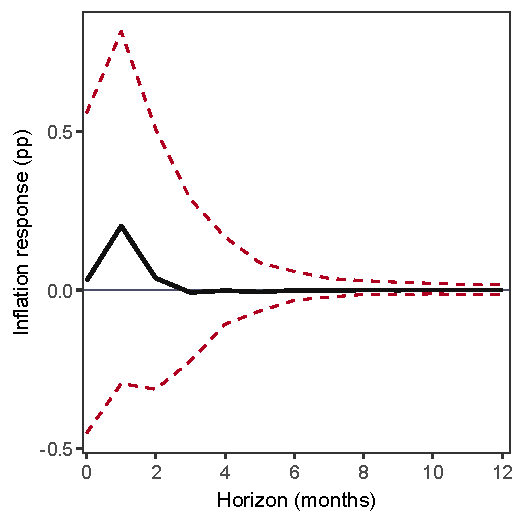
\includegraphics[width=\textwidth]{figures/tvar_girf_gold_normal.pdf}
    \caption{Non-Adverse Solvency-Growth State ($\Delta s_{t-1} > -4.615\%$)}
    \label{fig:tvar_girf_gold_normal}
\end{subfigure}
\hfill
\begin{subfigure}[b]{0.49\textwidth}
    \centering
    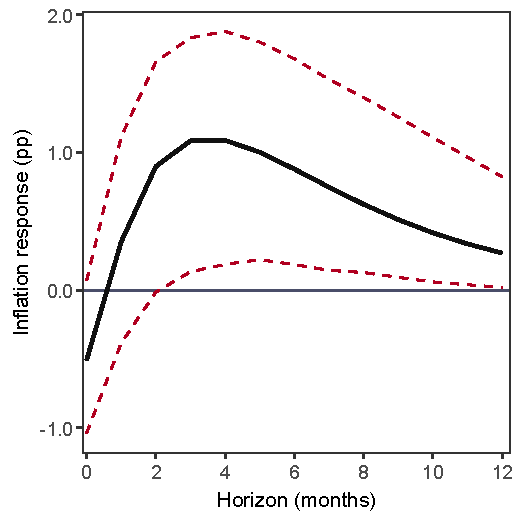
\includegraphics[width=\textwidth]{figures/tvar_girf_gold_insolv.pdf}
    \caption{Adverse Solvency-Growth State ($\Delta s_{t-1} \le -4.615\%$)}
    \label{fig:tvar_girf_gold_insolv}
\end{subfigure}
\caption{International Price Pass-Through across Solvency Regimes: The Dissolution of the External Buffer}
\label{fig:tvar_girf_gold_shield}
\begin{minipage}{\textwidth}
    \vspace{0.3em}
    \footnotesize \textbf{Notes:} Generalized Impulse Response Functions (GIRFs) of domestic consumer price inflation ($\pi_m$) to a one-standard-deviation structural shock in world gold price growth ($g^{gold}$) across solvency states. Solid black lines trace median bootstrap responses; dashed crimson lines represent 90\% empirical bootstrap confidence bands derived from 500 outer bootstrap replications and 1,000 inner Monte Carlo draws. The horizontal benchmark line marks zero. \textbf{Panel (A)} displays transmission in the non-adverse state ($\Delta s_{t-1} > -4.615\%$). \textbf{Panel (B)} displays transmission in the adverse solvency-growth state ($\Delta s_{t-1} \le -4.615\%$), reflecting conditions of central-bank insolvency.
\end{minipage}
\end{figure}

In the adverse solvency-growth state ($\Delta s_{t-1} \le -4.615\%$, Panel~B, reflecting conditions of central-bank insolvency), this insulation mechanism dissolves. The identical international price shock unleashes an unbroken 10-month inflationary wave ($h=3$ to $12$). Domestic inflation accelerates to a peak of $0.982$ percentage points at month 3 and delivers a cumulative price expansion of $6.542$ percentage points. The point-wise multiplier difference test ($\Delta_{g^{gold} \to \pi_m}(h)$) is strictly positive and statistically significant across all 10 consecutive months ($h=3$ to $12$), peaking at $+0.999$ percentage points at month 3. Adequate foreign reserves insulate the domestic economy; depleted reserves leave it vulnerable to international price shocks. When external commercial credit dried up and liquid reserves fell near zero, the state could no longer convert domestic currency into world money to stabilize import costs. International inflation transmitted directly into domestic consumer prices.

\paragraph{Cost-Push Inflation Inertia and Structural Imbalance Magnification.}
The non-linear transmission dynamics extend to domestic price persistence and real structural trade imbalances. In the non-adverse state, an unexpected domestic price shock ($\pi_m \to \pi_m$) accelerates monthly inflation by $3.786$ percentage points on impact, but dissipates steadily, losing statistical significance by month 7 with a cumulative effect of $6.459$ percentage points. In the adverse solvency-growth state, price momentum locks into the system: statistical significance persists across 11 consecutive months ($h=0$ to $10$), generating nearly double the cumulative price acceleration ($11.655$ percentage points). The persistence differential ($\Delta_{\pi_m \to \pi_m}(h)$) peaks at $+1.048$ percentage points at month 2 and maintains unbroken statistical significance for nine consecutive months ($h=2$ to $10$). In non-adverse periods, the state can damp distributive conflict by importing wage goods; under solvency distress, the inability to import turns every price shock into an entrenched markup struggle.

Real structural trade imbalance shocks ($\Delta\ln\Theta \to \Delta\ln\Theta$) likewise propagate asymmetrically. In the non-adverse state, the import-export gap displays monotonic decay ($+39.667$ percentage points on impact, cumulative $+24.523$ percentage points). In the adverse solvency-growth state, the initial imbalance ($+45.674$ percentage points) triggers an amplified oscillatory cycle. The regime differential peaks at $+15.364$ percentage points at month 1 and remains statistically significant across nine consecutive months ($h=1$ to $9$). Balance-of-payments distress destabilizes the physical import pipeline, creating recurring shortages of haul-truck tires, industrial replacement parts, and agricultural inputs rather than a smooth real adjustment. Finally, simulated regime-switching probabilities indicate that crossing between states is not driven by isolated monthly shocks: from the non-adverse state, the probability shift of crossing into the adverse state is negligible ($\Delta P \approx 0$). Once the system is in the adverse solvency-growth state ($\Delta s_{t-1} \le -4.615\%$, reflecting conditions of central-bank insolvency), favorable terms-of-trade shocks also produce negligible probability changes ($\Delta P \approx 0$). The simulated probability changes are negligible under these shocks, indicating persistence of the fitted adverse state over the reported horizon.



\subsubsection{Synthesis: Non-Linearity and the Peripheral Monetary Circuit}
\label{sec:tvar_synthesis}

\paragraph{Resolving the Nominal Paradox: Money as Consequence, Not Prime Mover.}
The regime-dependent parameter estimates resolve the central empirical puzzle of the Chilean inflation. Orthodox accounts treat the statistical correlation between base money growth and consumer price inflation during 1972--1973 as proof of an exogenous, printing-press-driven inflationary breakdown. Within the identified TVAR, the estimated response from inflation to base-money growth is more persistent and cumulatively larger under insolvency than the reverse response, more consistent with a substantial accommodation channel than with a purely autonomous-money interpretation. In the non-adverse state, base money growth accommodates inflation only modestly ($\hat{\beta} = 0.24$). In the adverse solvency-growth state ($\Delta s_{t-1} \le -4.615\%$, reflecting conditions of central-bank insolvency), accommodation surges to $\hat{\beta} = 0.58$ and inflation persistence jumps to $0.68$. The high observed correlation between money and prices reflects an endogenous consequence of structural solvency distress. The Central Bank expanded domestic liquidity to finance enterprise payrolls and prevent immediate liquidation, even as external supply ceased.

\paragraph{The Peripheral Monetary Circuit and the Hard-Currency Ceiling.}
These threshold dynamics illustrate the material limits of the peripheral monetary circuit. In an asymmetric international currency hierarchy, the state can issue domestic fiat liabilities, but it cannot manufacture world money. When foreign trade credit lines were severed and liquid reserves drained toward zero, the state could no longer convert domestic base money into essential imported machinery, spare parts, or food. Distributive conflict over real income could no longer be dampened through external supply. Under acute solvency depletion, domestic credit expansion dilutes external backing, leaving international price shocks unbuffered, generating persistent inflationary pressure, and inducing defensive monetization.

\paragraph{From Reserve Balance Sheets to the Political Economy of Subordination.}
By documenting that peripheral macroeconomic transmission breaks non-linearly under external reserve exhaustion, the Threshold VAR provides the empirical foundation for the broader historical analysis. Section~\ref{sec:discussion_conclusion} builds upon these findings to evaluate the political economy of the international credit blockade, organized distribution sabotage, and the institutional limits of peripheral monetary sovereignty.

